\section{Einleitung}
\label{chap:einleitung}

\subsection{Motivation und Projektziele}
Das vorliegende Projekt entstand im Rahmen des Moduls „Information Retrieval“ und diente der praktischen Anwendung der im Kurs vermittelten theoretischen Grundlagen. Die zentrale Aufgabenstellung bestand darin, eine eigenständige Suchanwendung auf Basis der etablierten Open-Source-Technologie Apache Solr zu konzipieren und umzusetzen.

Für die Umsetzung wurde die Pokémon API (pokeAPI.co) als Datenquelle ausgewählt. Auf dieser Grundlage entstand die Anwendung „Solr Pokédex“. Im Rahmen des Projekts wurden sowohl übergeordnete Ziele als auch konkrete funktionale Anforderungen definiert. Ein zentrales Ziel war die Entwicklung einer vollständigen Indexierungspipeline, die in der Lage ist, Daten automatisiert von der Quelle abzurufen, zu bereinigen und für Solr entsprechend aufzubereiten. Darüber hinaus sollte ein robustes und erweiterbares Solr-Schema entworfen werden, das die Struktur und Eigenschaften des gewählten Datensatzes sinnvoll abbildet. Für eine realistische und aussagekräftige Suchumgebung war die Indexierung eines relevanten Datenbestands vorgesehen, der mindestens 1000 einzigartige Einträge umfasst. Abgerundet wurde das Projektziel durch die Entwicklung einer simplen Weboberfläche, welche eine einfache und benutzerfreundliche Interaktion mit der Suchmaschine ermöglichen sollte.

\subsection{Funktionale Kernanforderungen}

Zur Erreichung der genannten Ziele musste die Anwendung bestimmte funktionale Anforderungen erfüllen. Dazu gehörte die Unterstützung verschiedener Suchanfragetypen, darunter eine klassische Keywordsuche über zentrale Textfelder, eine Phrasensuche zur gezielten Suche nach exakten Wortfolgen, eine Wildcardsuche mit Platzhaltern für flexible Suchmuster sowie eine facettierte Suche, die das Filtern von Ergebnissen nach Kriterien wie Pokémon-Typ oder Generation ermöglicht.

Um die Benutzerfreundlichkeit weiter zu erhöhen, wurden außerdem Funktionen zur Fehlerbehandlung und Ähnlichkeitssuche integriert. So sollte das System in der Lage sein, bei fehlerhaften Eingaben passende Korrekturvorschläge zu liefern („Meinten Sie…?“) und zusätzlich thematisch verwandte Inhalte zu einem Suchergebnis anzuzeigen („More like this“).

Über die funktionalen Kernanforderungen hinaus wurden einige optionale Erweiterungen als sogenannte „Stretch Goals“ formuliert. Dazu zählte unter anderem eine Autocompletion-Funktion, die während der Eingabe bereits passende Suchvorschläge anbietet, sowie ein Highlighting-Mechanismus, der die gesuchten Begriffe direkt in der Ergebnisvorschau visuell hervorhebt.

\subsection{Vorstellung der Suchmaschine Solr Pokédex}
\label{sec:vorstellung_pokedex}

Die im Rahmen dieses Projekts entwickelte Anwendung trägt den Namen „Solr Pokédex“ und ist eine spezialisierte Suchmaschine für Pokémon. Sie bietet einen umfassenden Index, der alle 1025 Pokémon der Generationen eins bis neun abdeckt.

Jedes Pokémon wird als eigenständiges Dokument in Apache Solr gespeichert und mit einer Vielzahl von detaillierten Metadaten angereichert. Diese Daten wurden sorgfältig ausgewählt, um sowohl eine gezielte Suche nach Fakten als auch eine explorative Volltextsuche zu ermöglichen. Zu den zentralen indexierten Feldern gehören:
\begin{itemize}
    \item \textbf{Stammdaten:} Name, Pokédex-ID, Typ(en), Generation, Größe und Gewicht.
    \item \textbf{Fähigkeiten und Kampfwerte:} Alle erlernbaren Fähigkeiten sowie die Basiswerte für Lebenspunkte (HP), Angriff, Verteidigung etc.
    \item \textbf{Beschreibender Text:} Ein separates Feld namens \texttt{flavor\_text} enthält die offiziellen Beschreibungen aus den Spielen. Mit seinem größeren Textumfang bildet dieses Feld die ideale Grundlage für eine freie Volltextsuche, die über die Suche nach reinen Fakten hinausgeht.
\end{itemize}

Die Interaktion mit der Suchmaschine erfolgt über eine mit Flask entwickelte Weboberfläche, die unter \texttt{http://localhost:5000} erreichbar ist. Die gesamte Anwendung ist containerisiert und lässt sich mittels Docker Compose und einem bereitgestellten Installationsskript (\texttt{install.sh}) unkompliziert einrichten und starten.

\subsection{Verwendeter Technologie-Stack}
\label{sec:tech_stack}

Die Architektur des „Solr Pokédex“ basiert auf einer Auswahl bewährter Open-Source-Technologien, die gezielt für ihre jeweilige Aufgabe im Projekt eingesetzt wurden. Der Stack lässt sich in die Bereiche Backend, Frontend, Datenquelle und Deployment unterteilen. Die prozentuale Verteilung der Programmiersprachen im Projekt (siehe Abbildung \ref{fig:language-distribution}) spiegelt diese Aufteilung wider.

\begin{figure}[h!]
\centering
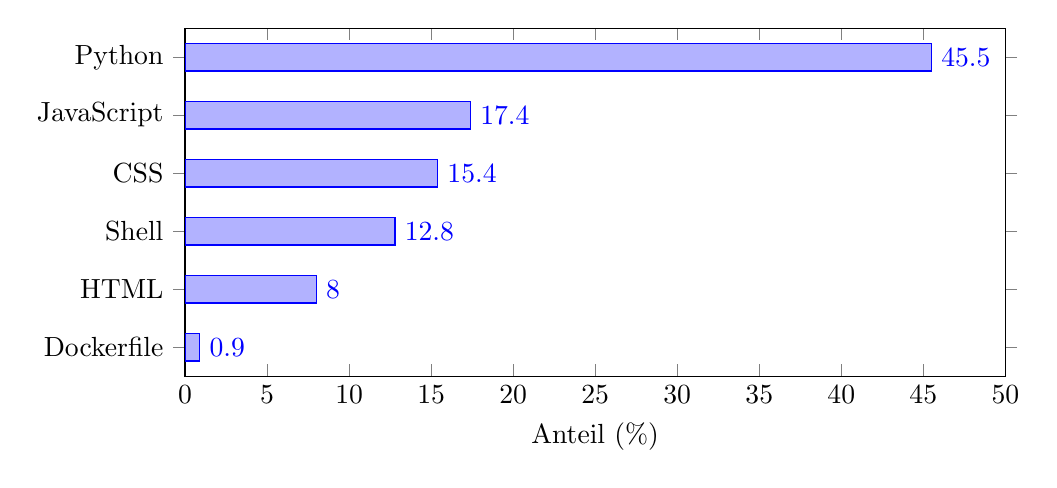
\begin{tikzpicture}
\begin{axis}[
    xbar,
    width=12cm,
    height=6cm,
    xlabel={Anteil (\%)},
    symbolic y coords={Dockerfile,HTML,Shell,CSS,JavaScript,Python},
    ytick=data,
    nodes near coords,
    nodes near coords align={horizontal},
    xmin=0,
    xmax=50
]
\addplot coordinates {
    (0.9,Dockerfile)
    (8.0,HTML)
    (12.8,Shell)
    (15.4,CSS)
    (17.4,JavaScript)
    (45.5,Python)
};
\end{axis}
\end{tikzpicture}
\caption{Sprachverteilung im Codebestand}
\label{fig:language-distribution}
\end{figure}


\paragraph{Backend und Datenverarbeitung (Python, Apache Solr)}
Das Herzstück der Anwendung bildet das Backend, das primär in \textbf{Python} implementiert ist. Python wurde aufgrund seiner exzellenten Bibliotheken für Webentwicklung und Datenverarbeitung sowie seiner einfachen Lesbarkeit gewählt.
\begin{itemize}
    \item \textbf{Apache Solr:} Als Suchserver-Technologie wurde Solr eingesetzt, da es in der Lehrveranstaltung als Standard vorgegeben war. Eine freie Wahl zwischen verschiedenen Suchmaschinen bestand daher nicht, auch wenn Alternativen wie OpenSearch oder Elasticsearch ebenfalls interessante Optionen gewesen wären. Dennoch überzeugt Solr durch eine hohe Performance, eine flexible Schema-Definition und eine mächtige Query-Syntax, was es zu einer geeigneten Grundlage für die Indexierung und komplexe Abfrage der Pokémon-Daten macht. Die Konfigurationen des Solr-Cores befinden sich im Verzeichnis \texttt{solr/configsets/}.
    
    \item \textbf{Flask}: Das leichtgewichtige Web-Framework Flask dient als Brücke zwischen dem Frontend und dem Solr-Server. Im Rahmen der Lehrveranstaltung wurde eine einfache Basisanwendung auf Grundlage von Flask bereitgestellt, welche ich für meine Anwendung entsprechend angepasst und erweitert habe. Die Datei \texttt{web/web\_app.py} verarbeitet die HTTP-Anfragen der Benutzeroberfläche, konstruiert die entsprechenden Solr-Queries und gibt die Ergebnisse als gerenderte HTML-Seite zurück.
    
    \item \textbf{Datenakquise:}
\end{itemize}
Zu Beginn entwickelte ich ein einzelnes, umfassendes Skript namens \texttt{fetcher\_v2.py}, das alle erforderlichen Funktionen zur Befüllung der Suchmaschine in sich vereinte. Mit der Zeit und der Implementierung zusätzlicher Features wuchs dieses Skript jedoch kontinuierlich an, bis es schließlich unübersichtlich und schwer wartbar wurde. Aus diesem Grund entschied ich mich für eine Refaktorierung und teilte das ursprüngliche Skript in mehrere spezialisierte Module auf:

\begin{itemize} \item \texttt{main.py}: Das Hauptskript, das den gesamten Datenabfrage- und Indexierungsprozess orchestriert \item \texttt{api\_client.py}: Verwaltet die Kommunikation mit der Pokemon API
\item \texttt{data\_processor.py}: Verarbeitet und transformiert die Pokemon-Daten für die Indexierung \item \texttt{solr\_indexer.py}: Übernimmt das Setup des Solr-Schemas und die Dokumentenindexierung \item \texttt{config.py}: Enthält Konfigurationseinstellungen und das Logging-Setup \end{itemize}

Das ursprüngliche Skript \texttt{fetcher\_v2.py} fungierte als zentrale Komponente zur Befüllung der Suchmaschine und übernahm sämtliche Aufgaben von der Konfiguration des Solr-Schemas über den Abruf der Daten von der PokeAPI bis hin zu deren Verarbeitung und finaler Indexierung. Es war so konzipiert, dass es auch auf einem frischen Solr-Core ohne manuelle Vorbereitung funktionsfähig war. Die Daten wurden systematisch bereinigt, angereichert und in eine für Solr optimierte Struktur überführt. Ein integrierter Batching-Mechanismus und eine detaillierte Protokollierung gewährleisteten dabei sowohl Effizienz als auch Transparenz im gesamten Indexierungsprozess. Eine detailliertere Beschreibung der einzelnen Komponenten und deren Funktionsweise folgt in den nachstehenden Kapiteln.

\paragraph{Frontend (HTML, CSS, JavaScript)}
Die Benutzeroberfläche wurde mit klassischen Web-Technologien realisiert, um eine einfache und reaktionsschnelle User Experience zu gewährleisten.
\begin{itemize}
    \item \textbf{HTML und CSS:} Die Struktur der Webseite ist in der Template-Datei \texttt{web/templates/index.html} definiert. Das Styling erfolgt über eine separate CSS-Datei (\texttt{web/static/style.css}).
    
    \item \textbf{JavaScript:} Für die dynamische Interaktivität auf der Client-Seite kommt pures JavaScript \texttt{web/\allowbreak static/\allowbreak js/\allowbreak main.js} zum Einsatz. Eine zentrale Funktion ist die Darstellung der Detailansicht eines Pokémon. Bei einem Klick auf ein Suchergebnis wird kein neuer Seitenaufruf ausgelöst. Stattdessen wird ein modales Fenster (Modal) über die bestehende Seite gelegt, das die Detailinformationen des ausgewählten Pokémon anzeigt. Dieser Ansatz verbessert die Benutzererfahrung, da der Kontext der Suchergebnisse erhalten bleibt.
\end{itemize}

\paragraph{Datenquelle}
Als externe Datengrundlage dient die \textbf{Pokémon API (pokeAPI.co)}. Sie bietet eine umfangreiche und gut strukturierte Sammlung von Pokémon-Daten im JSON-Format, die sich ideal für die Verarbeitung und Indexierung eignete.

\paragraph{Deployment und Automatisierung (Docker, Shell)}
Um eine einfache und reproduzierbare Einrichtung der Anwendung zu garantieren, wurde auf Containerisierung und Skripting gesetzt.
\begin{itemize}
    \item \textbf{Docker und Docker Compose:} Die gesamte Anwendung, inklusive des Solr-Servers und der Flask-App, wird durch die Datei \texttt{docker-compose.yml} als Multi-Container-Anwendung definiert. Dies isoliert die Komponenten und vereinfacht das Deployment erheblich.
    
    \item \textbf{Shell-Skripting:} Das Skript \texttt{install.sh} automatisiert den gesamten Setup-Prozess: Es richtet die Python-Umgebung ein, installiert Abhängigkeiten, startet die Docker-Container und initiiert die erstmalige Datenindexierung.
\end{itemize}